\documentclass[11pt]{article}
\usepackage[margin=2.3cm]{geometry}
\usepackage{booktabs}
\usepackage{amsmath}
\usepackage{xcolor}
\usepackage{array}
\usepackage{graphicx}
\usepackage{float}
\usepackage[font=small,labelfont=bf,skip=4pt]{caption}
\definecolor{darkblue}{RGB}{31,59,87}
\definecolor{goodgreen}{RGB}{47,143,78}
\definecolor{badred}{RGB}{179,45,45}
\definecolor{boxgray}{RGB}{243,244,246}
\setlength{\parskip}{4pt}
\setlength{\parindent}{0pt}
\newcommand{\qbox}[1]{\vspace{2pt}\noindent\colorbox{boxgray}{\parbox{\dimexpr\linewidth-2\fboxsep}{#1}}\vspace{3pt}}

\title{\color{darkblue}\textbf{What CPSS Does in Our CAS Pipeline}\\[2pt]
\large Simple explanation, with real clauses from our own run}
\author{}
\date{}

\begin{document}
\maketitle
\vspace{-1.5em}

\section*{0. The whole thing in one picture}

\begin{center}
\begin{tabular}{@{}c@{\;\;$\rightarrow$\;\;}c@{\;\;$\rightarrow$\;\;}c@{\;\;$\rightarrow$\;\;}c@{}}
\textbf{Trained TM} & \textbf{Basis $Z$} & \textbf{CPSS} & \textbf{Signature} \\
2{,}400 clauses & flows $\times$ clauses & vote over $2B$ halves & few stable clauses \\
(6 classes $\times$ 400) & 0/1 matrix & keep $\hat\pi_j\ge\pi_{\mathrm{thr}}$ & $S^+$ and $S^-$ \\
\end{tabular}
\end{center}

\qbox{\textbf{The idea in one line.} A clause can look useful by luck on one
split of the data. So we re-split the data many times, fit a sparse model
every time, and keep only the clauses that get picked \emph{again and again}.
That is CPSS --- Complementary-Pairs Stability Selection
(Shah \& Samworth, 2013).}

\section*{1. Which basis am I taking? (What goes into CPSS)}

This is the most important thing to get right: \textbf{CPSS does not look at
the raw network features at all.} The basis --- the columns of the matrix we
give to CPSS --- is the \textbf{clause activations}.

\begin{center}
\begin{tabular}{@{}lll@{}}
\toprule
 & Raw feature space & \textbf{Our basis $Z$ (what CPSS sees)} \\
\midrule
Columns  & 22 numeric flow features & 2{,}400 clauses ($6\times400$) \\
Values   & real numbers             & 0 or 1 (clause fired / did not fire) \\
Meaning  & ``Rate = 41{,}233 pkt/s'' & ``rule \#436 matched this flow'' \\
\bottomrule
\end{tabular}
\end{center}

So one row of $Z$ = one network flow. One column of $Z$ = one clause (one
learned rule). The entry is $z_{j}(x)\in\{0,1\}$.

\begin{figure}[H]\centering
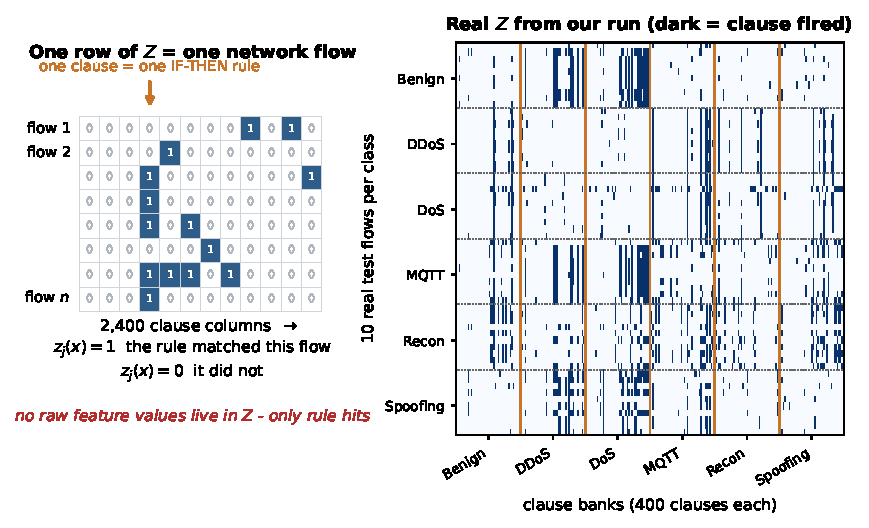
\includegraphics[width=\linewidth]{figs_explain/fig_z_anatomy.pdf}
\caption{\textbf{Left:} the shape of $Z$. \textbf{Right:} the real matrix from our seed-42 run --- 10 test flows per class (rows) against all 2{,}400 clauses (columns, split into the six banks by the orange lines). Each dark pixel is one clause firing on one flow. Flows of the same class light up recognisably similar column patterns: that pattern \emph{is} the signature CPSS goes looking for.}
\end{figure}

\subsection*{1a. So what does a clause activation actually contain?}

Nothing but a bit. $z_j(x)\in\{0,1\}$, and that is the whole content:
\emph{did rule $j$ match this flow, yes or no}. No confidence, no weight, no
feature value. The rule's weight $w_{c,j}$ and its reliability $\hat\pi_j$ live
elsewhere and are applied later.

Concretely, the object we hand to CPSS in our run is:

\begin{center}
\footnotesize
\begin{tabular}{@{}ll@{}}
\toprule
Property & Measured value (seed 42, test set) \\
\midrule
Shape & $80{,}868 \times 2{,}400$ (flows $\times$ clauses) \\
Storage type & \texttt{uint8}, $\approx$194\,MB \\
Values present & exactly $\{0,1\}$ --- nothing else \\
Clauses firing per flow & median \textbf{283} of 2{,}400 (min 138, mean 306, max 708) \\
Overall density & 12.8\% ones \\
Per-clause firing rate & median 5.6\%, 75th pct.\ 19.1\%, 90th pct.\ 44.1\% \\
Clauses that never fire & 817 of 2{,}400 (on a 20k-flow sample) \\
Clauses that always fire & 0 \\
\bottomrule
\end{tabular}
\end{center}

Two things follow from these numbers. First, $Z$ is \textbf{sparse but not
tiny}: about 300 rules match any given flow, so a flow is described by a
\emph{crowd} of overlapping rules, not one. Second, \textbf{a third of the
pool is dead weight} --- 817 clauses never fire at all, so they can never be
selected. This is exactly the redundancy that clause pruning removes.

\textbf{The columns have structure.} Column $j$ decodes as
$\text{bank} = \lfloor j/400\rfloor$ and, inside the bank, the first 200 are
\emph{positive-polarity} clauses (trained to fire on their own class) and the
last 200 are \emph{negative-polarity} (trained to fire on everything
\emph{except} their own class). That structure is visible in the raw counts:

\begin{figure}[H]\centering
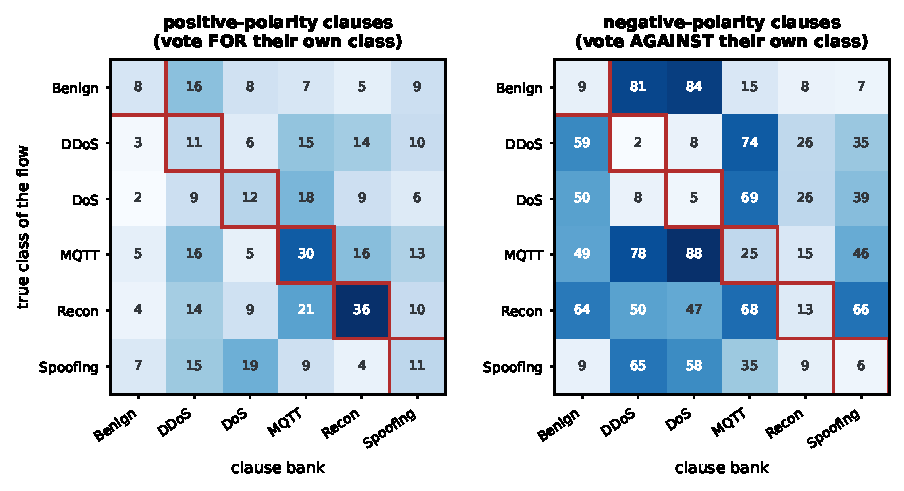
\includegraphics[width=\linewidth]{figs_explain/fig_banks.pdf}
\caption{Mean number of clauses firing per flow, by the flow's true class (rows) and the bank the clause came from (columns), out of 200 per half-bank. Red boxes mark the flow's own class. The negative-polarity half is near-silent on its own class --- Benign flows fire only 9 of Benign's 200 negative clauses but 81--84 of DDoS's and DoS's --- which is precisely what negative-polarity training is supposed to produce. Real data, 20{,}000 test flows.}
\end{figure}

\textbf{Why this basis and not the raw features?} Because we want the
explanation to be made of \emph{rules a human can read}, not of raw numbers.
Every column we select is already an IF-THEN rule (Section~6 shows how we
print it back out). Selecting features would give us ``Rate matters'';
selecting clauses gives us ``\emph{IF} Rate$\ge$bin7 \emph{AND NOT}
Header\_Length$\ge$bin4 \emph{THEN} DDoS''.

\textbf{One subtle point.} The pool is \emph{all} 2{,}400 clauses, not only
the 400 clauses of the class being explained. So the DDoS signature is
allowed to borrow a clause out of the Benign bank if that clause is a
reliable DDoS indicator. This really happens in our run (see Section~6).

\section*{2. What is $B$? (How the data is split)}

$B$ is the \textbf{number of complementary pairs}.

One ``complementary pair'' = shuffle the fit rows, cut them into two
\emph{disjoint} halves. Half~A and half~B together cover the data exactly
once, with no overlap --- that is what ``complementary'' means.

Do that $B$ times $\Rightarrow$ you get $2B$ halves in total.

\begin{center}
\begin{tabular}{@{}lll@{}}
\toprule
Pair & Half 1 & Half 2 (the complement) \\
\midrule
$b=1$ & rows \{3, 7, 8, \dots\} & rows \{1, 2, 4, \dots\} \\
$b=2$ & (new shuffle) rows \{1, 5, 9, \dots\} & rows \{2, 3, 6, \dots\} \\
$b=3$ & (new shuffle) \dots & \dots \\
\bottomrule
\end{tabular}
\end{center}

With $B=15$ we fit $2B=30$ half-models per class. A clause that survives all
30 different views of the data is genuinely stable; one that appeared only
because of a lucky subset will not.

\begin{figure}[H]\centering
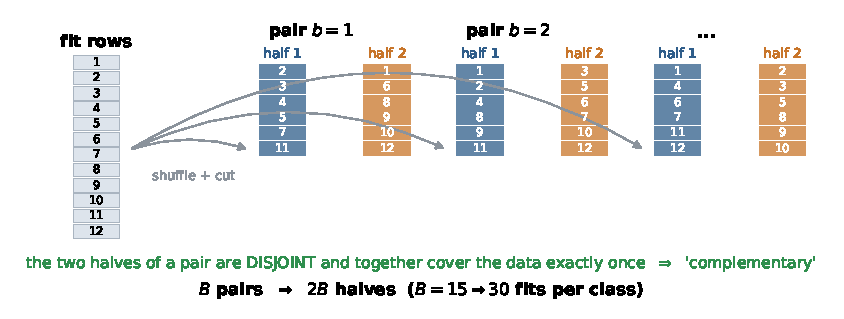
\includegraphics[width=\linewidth]{figs_explain/fig_pairs.pdf}
\caption{One complementary pair = one shuffle, cut into two disjoint halves. Repeat $B$ times to get $2B$ halves.}
\end{figure}

\qbox{\textbf{Why \emph{complementary} halves and not just random subsamples?}
Because the Shah--Samworth error bound in the paper (Eq.~9) is proved for
complementary pairs. If we used ordinary bootstrap resamples we would keep the
intuition but lose the bound. That is the only reason for the pairing.}

\textbf{What changes if I change $B$:} larger $B$ = more re-splits = the
stability score $\hat\pi_j$ is measured more finely (with $B=5$ the score can
only be $0, 0.1, 0.2, \dots, 1.0$; with $B=25$ it has 50 possible levels) and
is less noisy --- but it costs $2B\times6$ logistic fits per grid point. We
sweep $B\in\{5,10,15,20,25\}$ and pick $B$ on the \emph{selection} partition,
never on the report partition.

\section*{3. How is the fit done? (What happens inside one half)}

On \emph{each} of the $2B$ halves, for \emph{each} class $\ell$, we do this:

\begin{enumerate}
  \item \textbf{Make a one-vs-rest label.} For DDoS: $y=1$ if the flow is
        DDoS, else $y=0$.
  \item \textbf{Fit an $\ell_1$ logistic regression} of $y$ on the clause
        columns $Z$. Settings: \texttt{liblinear} solver,
        \texttt{class\_weight="balanced"} (so rare classes are not drowned
        out), \texttt{max\_iter=200}.
        The $\ell_1$ penalty pushes most of the 2{,}400 coefficients to
        \emph{exactly} zero --- so the fit itself is a selector: the clauses
        left with a non-zero coefficient are the ones it chose.
  \item \textbf{Repeat over 6 regularisation strengths}
        $\kappa \in \operatorname{geomspace}(0.001,0.1,6)$, on the
        \emph{same} half. Small $\kappa$ = strong penalty = very few clauses
        survive; large $\kappa$ = weaker penalty = more survive.
  \item \textbf{Union over the grid.} A clause counts as ``selected on this
        half'' if \emph{any} of the 6 fits gave it $|\beta| > \delta$, with
        $\delta=10^{-8}$. This means we never have to pick one magic
        $\kappa$ --- we ask ``does this clause survive at \emph{some}
        sensible sparsity level?''.
\end{enumerate}

\textbf{Count the votes.} For clause $j$ and class $\ell$:
\[
\hat\pi_{\ell j} \;=\; \frac{\text{number of the } 2B \text{ halves where clause } j \text{ was selected}}{2B}
\]
\textbf{Keep the stable ones.} $j$ enters the signature if
$\hat\pi_{\ell j}\ge\pi_{\mathrm{thr}}$
(we sweep $\pi_{\mathrm{thr}}\in\{0.5,\dots,0.9\}$; the multiclass run picks
$0.8$, i.e.\ selected in at least 24 of 30 halves).

\textbf{Read the sign.} Average the coefficient $\bar\beta_{\ell j}$ over all
halves and all 6 grid points (zeros included). Then
\[
S_\ell^+=\{j:\hat\pi_{\ell j}\ge\pi_{\mathrm{thr}},\ \bar\beta_{\ell j}>0\}
\quad\text{(evidence \emph{for})},\qquad
S_\ell^-=\{\dots,\ \bar\beta_{\ell j}<0\}
\quad\text{(evidence \emph{against})}.
\]

\begin{figure}[H]\centering
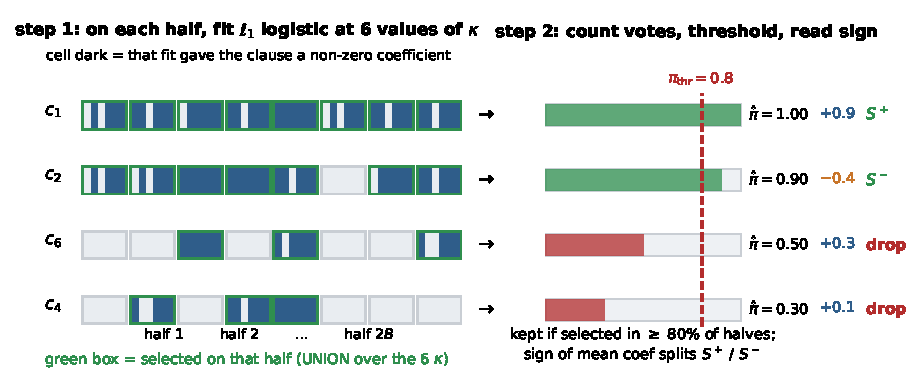
\includegraphics[width=\linewidth]{figs_explain/fig_vote.pdf}
\caption{The selection machinery end to end. \textbf{Left:} each of the $2B$ halves is fitted at six values of $\kappa$; a clause counts as selected on that half (green box) if \emph{any} of the six fits keeps it. \textbf{Right:} the vote fraction $\hat\pi_j$ is thresholded, and the sign of the mean coefficient sorts survivors into $S^+$ and $S^-$. Numbers match the toy example in Section~4.}
\end{figure}

\section*{4. Worked toy example (tiny numbers, made up for clarity)}

Imagine only \textbf{6 clauses}, $B=5$ pairs (so 10 halves),
and threshold $\pi_{\mathrm{thr}} = 0.8$. Class = DDoS.

\vspace{4pt}
\begin{center}
\begin{tabular}{@{}lccccl@{}}
\toprule
Clause & Selected in & $\hat\pi_j$ & Mean coef.\ & Keep? & Meaning \\
\midrule
$c_1$: high packet rate AND TCP & 10/10 & 1.0 & $+$0.9 &
  \textcolor{goodgreen}{\textbf{YES}} & supports DDoS \\
$c_2$: many unique dst ports    & 9/10  & 0.9 & $-$0.4 &
  \textcolor{goodgreen}{\textbf{YES}} & speaks against DDoS \\
$c_3$: dst port = 1883 (MQTT)   & 9/10  & 0.9 & $-$0.6 &
  \textcolor{goodgreen}{\textbf{YES}} & speaks against DDoS \\
$c_4$: small packets AND UDP    & 3/10  & 0.3 & $+$0.1 &
  \textcolor{badred}{no} & unstable, drop \\
$c_5$: long flow duration       & 2/10  & 0.2 & $+$0.2 &
  \textcolor{badred}{no} & unstable, drop \\
$c_6$: src port is random       & 5/10  & 0.5 & $+$0.3 &
  \textcolor{badred}{no} & coin-flip, not stable enough \\
\bottomrule
\end{tabular}
\end{center}

\vspace{2pt}
Result: DDoS signature $= S^+ = \{c_1\}$, $S^- = \{c_2, c_3\}$.
$c_6$ was picked half the time --- better than nothing, but a clause we
cannot reproduce is a clause we cannot testify with, so it is dropped.

\section*{5. How a new flow is scored}

A new flow $x$ arrives. We check which signature clauses fire on it:
\[
s_{\ell}(x)=
\frac{\displaystyle\sum_{j\in S_\ell^+}\hat\pi_j\,z_j(x)
      \;-\;\sum_{j\in S_\ell^-}\hat\pi_j\,z_j(x)}
     {\displaystyle\sum_{j\in S_\ell^+}\hat\pi_j}
\]
Each clause votes with its \emph{own reliability} $\hat\pi_j$ as the weight,
and the denominator normalises so that classes with big signatures are not
automatically favoured.

\textbf{Example (toy numbers above):} on flow $x$, $c_1$ fires ($z_1{=}1$),
$c_2$ does not ($z_2{=}0$), $c_3$ fires ($z_3{=}1$):
\[
s_{\text{DDoS}}(x)=\frac{(1.0)(1)-(0.9)(0)-(0.9)(1)}{1.0}
=\frac{1.0-0.9}{1.0}=0.1
\]
We compute this for all 6 families and take the largest. Every point of the
score traces back to a printable rule.

\section*{6. How do I get the rules back out?}

CPSS returns \emph{column indices}, e.g.\ ``clause 436''. Turning an index
back into a readable rule is two steps
(\texttt{scripts/decode\_signatures.py}):

\begin{enumerate}
  \item \textbf{Index $\rightarrow$ bank.} With $K=400$ clauses per class,
        $j=436$ means source class $\lfloor 436/400\rfloor = 1$ (DDoS) and
        clause 36 inside that bank. Clauses in the first half of a bank are
        \emph{positive-polarity}, the second half \emph{negative-polarity}.
  \item \textbf{TA states $\rightarrow$ literals.} We read
        \texttt{clause\_banks[c].get\_literals()}. Each clause is a row of
        $2\times154$ bits: bit $i$ on means the literal
        \texttt{feature>=bin$k$} is included; bit $154+i$ on means
        \texttt{NOT(feature>=bin$k$)} is included. The clause is the
        \textbf{AND} of everything included.
\end{enumerate}

\textbf{Real examples from our run} (seed 42, $\pi_{\mathrm{thr}}=0.8$,
DDoS signature):

\begin{center}
\footnotesize
\begin{tabular}{@{}p{0.30\textwidth}ccp{0.42\textwidth}@{}}
\toprule
Clause & $\hat\pi_j$ & $\bar\beta$ & Rule \\
\midrule
\#436, DDoS bank, positive & 1.00 & $+0.451$ &
IF \texttt{Rate>=bin7} AND \texttt{NOT(Header\_Length>=bin4)} \\
\#438, DDoS bank, positive & 1.00 & $+0.128$ &
IF \texttt{Rate>=bin5} AND \texttt{syn\_flag\_number>=bin1} AND \texttt{rst\_flag\_number>=bin1} \\
\#270, \textbf{Benign} bank, negative & 1.00 & $+0.045$ &
IF \texttt{Rate>=bin6} \quad\emph{(a clause borrowed from another class's bank)} \\
\bottomrule
\end{tabular}
\end{center}

Read clause \#436 in plain words: \emph{very high packet rate with a small header}
--- which is exactly what a flooding attack looks like. That is the kind of
sentence we can put in front of a clinician or an auditor.

\section*{7. What if clause $c_1$ has many literals?}

Short answer, in two parts.

\qbox{\textbf{(a) CPSS does not care at all.} CPSS only ever sees the column
$z_j\in\{0,1\}^n$. Whether that 0/1 came from a 2-literal rule or a
130-literal rule is invisible to the $\ell_1$ fit. A long clause is neither
penalised nor rewarded by the selection --- literal count only matters
\emph{afterwards}, when we print the rule for a human.}

\textbf{(b) A long clause is not really long --- it collapses.} The
thermometer encoding is cumulative
(\texttt{x>=bin1}, \texttt{x>=bin2}, \dots), so many literals on the
\emph{same} feature merge into one interval:
\[
\underbrace{\texttt{H>=bin2} \wedge \texttt{H>=bin3}}_{\text{keep the strongest: } \texttt{H>=bin3}}
\wedge
\underbrace{\neg\texttt{H>=bin4} \wedge \neg\texttt{H>=bin5} \wedge \dots}_{\text{keep the weakest: } \texttt{H<bin4}}
\;\;\Longrightarrow\;\;
\texttt{bin3} \le \texttt{Header\_Length} < \texttt{bin4}
\]

\begin{figure}[H]\centering
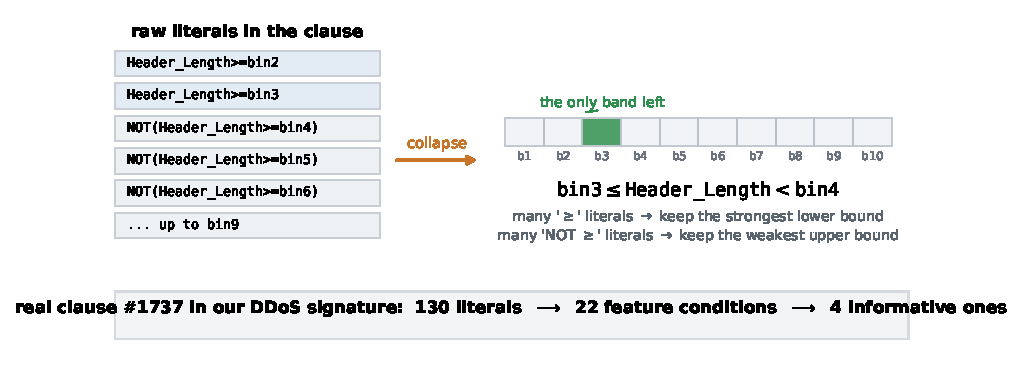
\includegraphics[width=\linewidth]{figs_explain/fig_collapse.pdf}
\caption{Why a long clause is not really long: cumulative thermometer bits on the same feature merge into a single interval.}
\end{figure}

\textbf{Real case from our run.} The longest clause in the seed-42 DDoS
signature is \#1737 (from the \emph{Recon} bank, $\hat\pi=0.967$,
$\bar\beta=+0.133$) with \textbf{130 literals}. After collapsing, those 130
literals are just \textbf{22 feature conditions}, and only four of them carry
information:

\begin{center}
\footnotesize
\begin{tabular}{@{}ll@{}}
\toprule
Collapsed condition & Reading \\
\midrule
\texttt{bin3 <= Header\_Length < bin4} & a narrow header-length band \\
\texttt{bin1 <= Protocol Type < bin2}  & one specific protocol \\
\texttt{Rate >= bin2}                  & at least moderate packet rate \\
\texttt{bin2 <= syn\_flag\_number < bin3} & a specific SYN count \\
\midrule
\parbox[t]{0.40\textwidth}{\texttt{ARP, DNS, HTTP, HTTPS, ICMP, SSH,\\
Telnet, SMTP, IRC, IGMP, DHCP,\\
fin/ack/psh/cwr/ece\_flag\_number,\\
rst\_count, rst\_flag\_number} all $=$ off}
& \parbox[t]{0.42\textwidth}{18 ``this protocol/flag is \textbf{off}'' conditions --- i.e.\ ``it is none of these other things''} \\[2pt]
\bottomrule
\end{tabular}
\end{center}

So ``130 literals'' really reads as: \emph{a moderate-rate flow, one specific
protocol, a narrow header band, a specific SYN count, and none of the common
application protocols or other TCP flags set.} Long, but still a sentence.

\textbf{How long are our clauses in practice?} Inculpatory signature clauses,
seed 42, $\pi_{\mathrm{thr}}=0.8$:

\begin{center}
\footnotesize
\begin{tabular}{@{}lcccc@{}}
\toprule
Class & \#clauses & shortest & \textbf{median} & longest \\
\midrule
Benign   & 41 & 1 & 5   & 153 \\
DDoS     & 29 & 1 & 2   & 130 \\
DoS      & 33 & 2 & 7   & 119 \\
MQTT     & 53 & 1 & 2   & 18  \\
Recon    & 28 & 1 & 3   & 132 \\
Spoofing & 50 & 1 & 1.5 & 153 \\
\bottomrule
\end{tabular}
\end{center}

The \emph{typical} signature clause is 1--7 literals. Long clauses exist but
they are the tail, not the rule. (The hard ceiling is $2\times154=308$
literals: 154 thermometer bits plus their negations.)

\textbf{The one real cost of a long clause.} It is very \emph{specific}, so
it fires on few flows. That is fine for stability --- it can still be
selected in all 30 halves if it fires consistently on that family --- but it
contributes to fewer decisions. Short clauses are the workhorses; long
clauses are the sharp corner cases.

\section*{8. The exact settings we use}

\begin{center}
\footnotesize
\begin{tabular}{@{}lll@{}}
\toprule
Quantity & Value & Where \\
\midrule
Clause pool $p$ & 2{,}400 ($6\times K$, $K=400$) & TM: $T=320$, $s=8$, 25 epochs \\
Boolean input & 154 bits (22 features $\times$ up to 10 quantile bins) & \texttt{data\_prep.py} \\
CPSS fit rows & 40{,}434 & fixed permutation, seed 0 \\
Selection rows & 20{,}217 & where $(B,\pi_{\mathrm{thr}})$ is chosen \\
Report rows & 20{,}217 & never touched until the final number \\
$B$ grid & $\{5,10,15,20,25\}$ & multiclass picks $B=15$ \\
$\pi_{\mathrm{thr}}$ grid & $\{0.5,0.6,0.7,0.8,0.9\}$ & multiclass picks $0.8$ \\
$\kappa$ grid $\Lambda$ & $\operatorname{geomspace}(0.001,0.1,6)$ & union over the grid \\
Zero tolerance $\delta$ & $10^{-8}$ & $|\beta|>\delta$ counts as selected \\
Logistic fit & liblinear, $\ell_1$, balanced, 200 iters & \texttt{stabilis.py} \\
\bottomrule
\end{tabular}
\end{center}

The three partitions are disjoint on purpose: CPSS \emph{fits} on one,
$(B,\pi_{\mathrm{thr}})$ is \emph{chosen} on the second, and the reported
macro-F1 comes from the third. Choosing the operating point on the same rows
we report on would be cheating.

\section*{9. Where each step lives}

\begin{center}
\footnotesize
\begin{tabular}{@{}lll@{}}
\toprule
Step & Code & Paper \\
\midrule
Build the basis $Z$      & \texttt{tm.transform(X)} & Sec.~II-A, Eq.~(1)--(2) \\
Shuffle + split halves   & \texttt{cpss\_proportions()}, \texttt{stabilis.py} & Sec.~II-C \\
$\ell_1$ logistic fit    & \texttt{cpss\_proportions()} & Sec.~II-C \\
Union over 6 $\kappa$    & \texttt{cpss\_proportions()} & Eq.~(6) \\
Vote count $\hat\pi_j$   & \texttt{cpss\_proportions()} & Eq.~(6) \\
Threshold + sign split   & \texttt{build\_signatures()} & Eq.~(7) \\
Attribution score        & \texttt{attribution\_scores()} & Eq.~(8) \\
Error-bound diagnostic   & \texttt{error\_bound()} & Eq.~(9) \\
Decode index $\to$ rule  & \texttt{decode\_signatures.py} & Sec.~IV \\
\bottomrule
\end{tabular}
\end{center}

\section*{10. One-paragraph summary}

\begin{quote}
\emph{We take the trained TM's 2{,}400 clauses as our basis: each clause is a
readable IF-THEN rule, and each flow becomes a 0/1 vector saying which rules
matched. For each attack family we split the fit data into $B$ complementary
pairs ($2B$ halves), run a sparse $\ell_1$ logistic fit on every half at six
regularisation strengths, and count how often each clause is picked. Clauses
picked in at least $\pi_{\mathrm{thr}}$ of the halves become the family's
signature; the sign of their average coefficient splits them into evidence
for ($S^+$) and evidence against ($S^-$). A new flow is scored by its signed,
reliability-weighted matches. Finally we decode each selected index back into
its literal conjunction --- typically 1--7 literals, and even a 130-literal
clause collapses to about 22 readable feature conditions.}
\end{quote}

\end{document}
